% Emacs, this is -*-latex-*-

\title{Energy Concentration and Spatial Multiresolution with the Discrete Wavelet Transform}

\maketitle
\tableofcontents
     
\section{The transform}

Technically, the
\href{https://en.wikipedia.org/wiki/Discrete_wavelet_transform}{DWT
  (Discrete Wavelet Transform)} is a
\href{https://en.wikipedia.org/wiki/Linearity}{linear}
\href{https://en.wikipedia.org/wiki/Change_of_basis}{basis}
\href{https://www.youtube.com/watch?v=P2LTAUO1TdA}{expansion} which
computes a
\href{https://www.dsprelated.com/freebooks/sasp/Critically_Sampled_Perfect_Reconstruction.html}{critically}-\href{https://en.wikipedia.org/wiki/Nyquist-Shannon_sampling_theorem}{sampled}
\href{https://en.wikipedia.org/wiki/Octave_(electronics)}{octave}-\href{https://en.wikipedia.org/wiki/Frequency_band}{band}
\href{https://www.sciencedirect.com/topics/engineering/wavelet-decomposition}{decomposition}~\cite{vetterli2014foundations,kovacevic2013fourier}. As the rest of transforms:
\begin{enumerate}
\item The output of the DWT describes the (input) signal in a set of
  \href{https://en.wikipedia.org/wiki/Sub-band_coding}{subbands},
  producing the so called a
  \href{https://en.wikipedia.org/wiki/Discrete_wavelet_transform}{decomposition}.
\item The
  \href{https://en.wikipedia.org/wiki/Array_data_structure#Element_identifier_and_addressing_formulas}{index}
  of the subband is related to the
  \href{https://en.wikipedia.org/wiki/Frequency}{frequency} of the
  signal. For example, in the case of the
  \href{https://en.wikipedia.org/wiki/Digital_image}{images}, the
  position of the
  \href{https://en.wikipedia.org/wiki/Coefficient}{coefficients} in
  the subbands is related to
  \href{https://en.wikipedia.org/wiki/Discrete_wavelet_transform#/media/File:Jpeg2000_2-level_wavelet_transform-lichtenstein.png}{the
    spatial area where the corresponding pixels are found}.
\end{enumerate}

\subsection{1D case}

The 1D-DWT convolves the input signal with a set of basis functions
(you can see the basis functions of several DWTs in the
\href{http://wavelets.pybytes.com/}{Wavelet Browser}) defined by a
\href{https://tecnologias-multimedia.github.io/milestones/12-temporal_coding/}{cascade
  of filters banks}, building a dyadic signal decomposition in the
frequency domain.

\subsubsection{An example of DWT: the Haar DWT}
The DWT is also described by the filters of
the analysis matrix transform (the matrix ${\mathbf K}$ in previous
  milestones). Haar defined the analysis
\href{https://en.wikipedia.org/wiki/Downsampling_(signal_processing)}{downsampling}
filters
\begin{equation}
  \begin{bmatrix}
    {\mathbf l}^{s+1}_n \\
    {\mathbf h}^{s+1}_n
  \end{bmatrix}
  = 
  \begin{bmatrix} \frac{1}{\sqrt{2}} & \frac{1}{\sqrt{2}} \\ \frac{1}{\sqrt{2}} & \frac{-1}{\sqrt{2}} \end{bmatrix}
  \begin{bmatrix}
    {\mathbf l}^s_{2n} \\
    {\mathbf l}^s_{2n+1}
  \end{bmatrix},
  \label{eq:Haar_transform}
\end{equation}
where the superindex $s$ denotes the subband, and $n$ refers to the
$n$-th element of the signal. By definition (and notice that this
holds for all DWTs),
\begin{equation}
  {\mathbf l}^0={\mathbf x}.
\end{equation}

\begin{figure}
  \centering
  \svgfig{graphics/haar_modulus}{6cm}{600}
  \caption{Haar filters's response in the frequency domain (see this
    \href{https://github.com/Sistemas-Multimedia/Sistemas-Multimedia.github.io/blob/master/milestones/08-DWT/DWT_filters_analysis.ipynb}{notebook}).
    $|{\mathbf K}_i(e^{j\omega})|$ denotes the
    \href{https://en.wikipedia.org/wiki/Absolute_value}{modulus} of
    the \href{https://en.wikipedia.org/wiki/Fourier_transform}{Fourier
      transform} of ${\mathbf K}_i$.}
  \label{fig:Haar_modulus}
\end{figure}

\begin{figure}
  \centering
  \svgfig{graphics/db5_modulus}{6cm}{600}
  \caption{Daubechies-5 filters's response in the frequency domain
    (see this
    \href{https://github.com/Sistemas-Multimedia/Sistemas-Multimedia.github.io/blob/master/milestones/08-DWT/DWT_filters_analysis.ipynb}{notebook}).}
  \label{fig:db5_modulus}
\end{figure}

\begin{figure}
  \centering
  \svgfig{graphics/bior3.5_modulus}{6cm}{600}
  \caption{Biorthiogonal-3.5 filters's response in the frequency
    domain (see this
    \href{https://github.com/Sistemas-Multimedia/Sistemas-Multimedia.github.io/blob/master/milestones/08-DWT/DWT_filters_analysis.ipynb}{notebook}).}
  \label{fig:bior3.5_modulus}
\end{figure}

\begin{figure}
  \centering
  \svgfig{graphics/haar_phase}{6cm}{600}
  \caption{Phase response of the Haar filters (see this
    \href{https://github.com/Sistemas-Multimedia/Sistemas-Multimedia.github.io/blob/master/milestones/08-DWT/DWTfilters_analysis.ipynb}{notebook}).}
  \label{fig:haar_phase}
\end{figure}

\begin{figure}
  \centering
  \svgfig{graphics/db5_phase}{6cm}{600}
  \caption{Phase response of the Daubechies-5 filters (see the
    notebook
    \href{https://github.com/vicente-gonzalez-ruiz/DWT/blob/master/docs/graphics/DWT_filters_study.ipynb}{Study
      of some wavelet filters}). Notice that we obtained phase
    responses are not completely linear (it is not a straight line).}
  \label{fig:db5_phase}
\end{figure}

As it can be seen in the Fig.~\ref{fig:Haar_modulus}, ${\mathbf K}_0$ is a
\href{https://en.wikipedia.org/wiki/Low-pass_filter}{low-pass filter}
and ${\mathbf K}_1$ is a
\href{https://en.wikipedia.org/wiki/High-pass_filter}{high-pass
  filter} (this holds for all DWTs). Considering the Haar filter, we
can conclude that:
\begin{enumerate}
\item There exists
  \href{https://en.wikipedia.org/wiki/Aliasing}{aliasing} between the
  filters (this is also true for all DWTs) and this is a drawback
  because: \begin{enumerate} \item The same
    \href{https://en.wikipedia.org/wiki/Information}{information} can
    be found in both subbands (${\mathbf l}$ and ${\mathbf
      h}$). Therefore, the concentration of the energy in one of the
    subbands is smaller.
  \item As it can be seen also in Eq.~\eqref{eq:Haar_transform}, the
    subbands are downsampled by 2 (action usually represented by
    $\downarrow 2$) and both subbands should have, at most, a
    \href{https://en.wikipedia.org/wiki/Bandwidth_(signal_processing)}{bandwidth}
    of $\frac{1}{2}$
    \href{https://en.wikipedia.org/wiki/Radian}{radians}/\href{https://en.wikipedia.org/wiki/Sampling_(signal_processing)}{sample}
    in order to avoid the aliasing during the
    \href{https://en.wikipedia.org/wiki/Downsampling_(signal_processing)}{subsampling},
    thus increasing the
    \href{https://en.wikipedia.org/wiki/Perception}{perceptible}
    \href{https://en.wikipedia.org/wiki/Signal-to-noise_ratio}{quality}
    of the low-pass subband ${\mathbf l}$.  \end{enumerate} These
  problems can be only solved using filters that have
  \href{https://en.wikipedia.org/wiki/Transfer_function}{transfer
    functions} that overlaps a smaller area\footnote{Sharper
  transition bands.} (see Figs.~\ref{fig:db5_modulus} and
  \ref{fig:bior3.5_modulus}).
%\item The response of the filter bank is flat, which means that the gain of the different frequencie
%  $|y(e^{j\omega})|=a|x(e^{j\omega})|, a\in\mathbb{R}$ (the
%  reconstructed signal $y$ has not been filtered). % OJO
\item There is not
  \href{https://en.wikipedia.org/wiki/Linear_phase}{phase distortion}
  (the phase of the filters is a linear function of the frequency, see
  the Fig.~\ref{fig:haar_phase}). This means that both coefficients
  ${\mathbf l}^{s+1}_n$ and ${\mathbf h}^{s+1}_n$ refers to the same section of signal
  $\{{\mathbf l}^s_{2n}, {\mathbf l}^s_{2n+1}\}$, allowing the design of entropy codecs
  for the decomposition which exploit the correlation between
  subbands. Notice that this does not hold for all filters (see
  Fig.~\ref{fig:db5_phase}).
\end{enumerate}

% Polyphase implementation of the multilevel DWT
\begin{figure}
  \centering
  \svgfig{graphics/DWT}{4cm}{400}
  %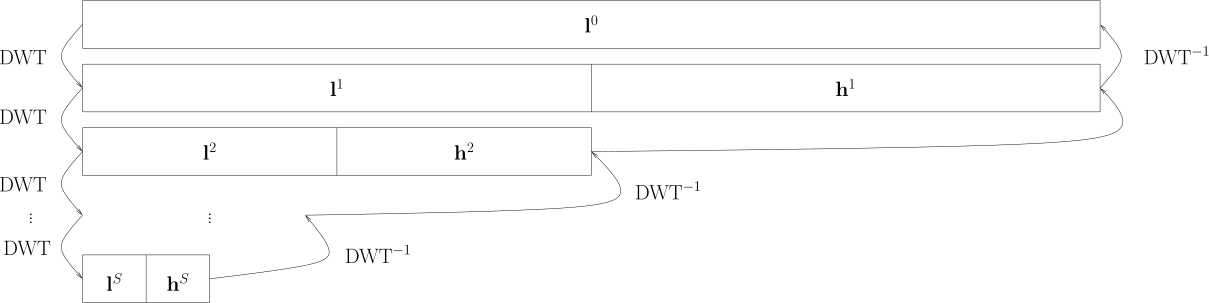
\includegraphics[width=0.8\textwidth]{graphics/DWT}
  %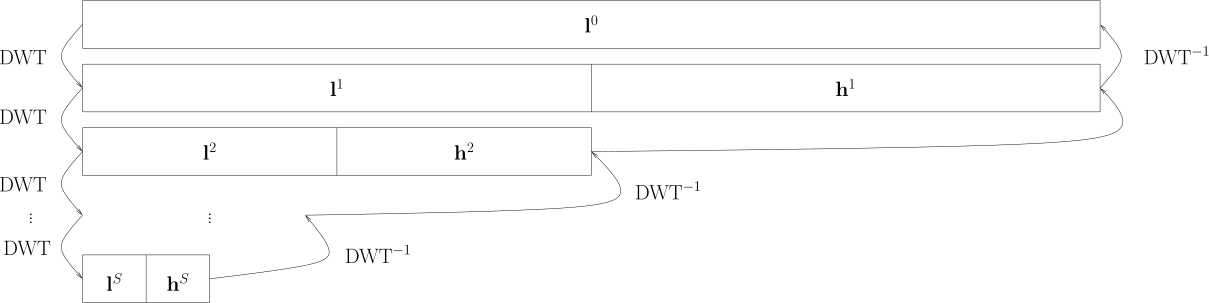
\includegraphics[width=4cm]{graphics/DWT}
  %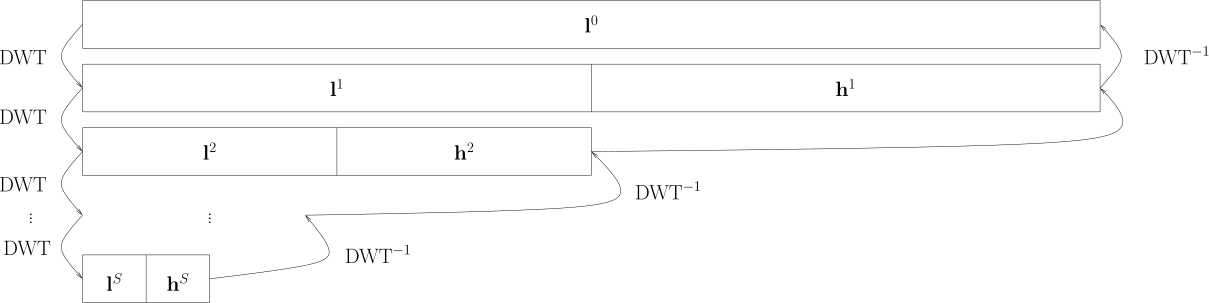
\includegraphics{graphics/DWT}
  \caption{Computation of the $S$-levels DWT and the generated
    subbands.}
  \label{fig:DWT}
\end{figure}

Eq.~\eqref{eq:Haar_transform} computes the 1-levels Haar DWT. A more
general expresion for this equation (and this holds for all DWTs) is
\begin{equation}
  {\mathbf l}^{s+1} | {\mathbf h}^{s+1} = \text{DWT}({\mathbf l}^s),
  \label{eq:DWT}
\end{equation}
where $\cdot|\cdot$ denotes the concatenation of subbands. As can
be seen in the Fig.~\ref{fig:DWT}, it's possible to compute the
$S$-levels DWT, using Eq.~\eqref{eq:DWT} iteratively over the
low-frequency subband, generating the decomposition
\begin{equation}
  {\mathbf l}^S_0 | {\mathbf h}^S_0 | {\mathbf h}^{S-1}_0 {\mathbf
    h}^{S-1}_1 | {\mathbf h}^{S-2}_0 {\mathbf h}^{S-2}_1 {\mathbf
    h}^{S-2}_2 {\mathbf h}^{S-2}_3 | \cdots | {\mathbf h}^1_0 h^1_1
  \cdots {\mathbf h}^1_{2^{n-1}-1}=\text{DWT}^S({\mathbf l}^0),
  \label{eq:S_levels_DWT}
\end{equation}
where
\begin{equation}
  n = \log_2(N)
\end{equation}
where $N$ is the number of samples.

In the case of the Haar filters, the synthesis (inverse) $1$-levels
DWT (that we will denote by $\text{DWT}^{-1}$) is the result of
solving the coefficients ${\mathbf l}^{s+1}_n$ and ${\mathbf h}^{s+1}_n$ in the
Eq.~\eqref{eq:Haar_transform}. In general, for longer DWT filters we are
going to have more coefficients, but the same procedure can be used
for finding the synthesis transform. Therefore, it can be written that
\begin{equation}
  {\mathbf l}^s = \text{DWT}^{-1}({\mathbf l}^{s+1} | {\mathbf h}^{s+1}),
\end{equation}
and $\text{DWT}^{-S}$, the $S$-levels synthesis DWT, can be computed
as it is also described in the Fig.~\ref{fig:DWT}, by simply reversing
the analysis steps.

\subsubsection{\href{https://en.wikipedia.org/wiki/Multiresolution_analysis}{Multiresolution analysis}}
In the decomposition described in Eq.~\eqref{eq:S_levels_DWT} there are
$S+1$ subbands, and therefore, it is possible to compute $S+1$
resolution levels of the analyzed signal ${\mathbf l}^0$:
\begin{itemize}
\item  ${\mathbf l}^S$: the resolution level $S$ of ${\mathbf l}^0$ (no $\text{DWT}^{-1}$ has been
  applied in the synthesis process), with have only one sample ${\mathbf l}^S_0$ that uses to be the
  \href{https://en.wikipedia.org/wiki/Arithmetic_mean}{arithmetic
    mean} of ${\mathbf l}^0$. The coefficient ${\mathbf l}^S_0$
  is also called the \href{https://en.wikipedia.org/wiki/DC_bias}{DC
    (Direct Current) coefficient}. On the contrary, the rest of
  coefficents (high-frequency subbands) are called the AC (Alternating
  Current) coefficients.
\item ${\mathbf l}^{S-1}=\text{DWT}^{-1}({\mathbf l}^S | {\mathbf
  h}^S)$, the resolution level $S-1$ of ${\mathbf l}^0$, with two
  samples.
\item ${\mathbf l}^{S-2}=\text{DWT}^{-1}({\mathbf l}^{S-1} | {\mathbf
  h}^{S-1})$, the resolution level $S-1$ of ${\mathbf l}^0$, with
  four samples.
\item $\vdots$
\item The resolution level $0$, ${\mathbf
  l}^0=\text{DWT}^{-1}({\mathbf l}^1 | {\mathbf h}^1)$.
\end{itemize}  

\subsubsection{Filters}

\begin{figure}
  \centering
  \svgfig{graphics/PRFB}{4cm}{400}
  \caption{A 2-channels PRFB (Perfect Reconstruction Filter Bank). See
    the notebook
    \href{https://github.com/vicente-gonzalez-ruiz/DWT/blob/master/docs/PRFB.ipynb}{A
      Perfect Reconstruction Filter Bank (PRFB)}.}
  \label{fig:PRFB}
\end{figure}

All DWTs are defined by 4 filters (using a similar notation that the
followed by \href{https://pywavelets.readthedocs.io}{PyWavelets}) (see
Fig.~\ref{fig:PRFB}):
\begin{enumerate}
\item Analysis (downsampling) low-pass filter $\tilde\phi$ (the
  decomposition scaling function), which computes ${\mathbf l}^{s+1}$
  from ${\mathbf l}^s$.
\item Analysis (downsampling) high-pass filter $\tilde\psi$ (the
  decomposition wavelet function), which computes ${\mathbf h}^{s+1}$
  from ${\mathbf l}^s$.
\item Synthesis (upsampling) high-pass filter $\phi$ (the
  reconstruction scaling function), which computes $\{{\mathbf
    l}^s_{2n}\}$ from ${\mathbf l}^{s+1}$ and ${\mathbf h}^{s+1}$.
\item Synthesis (upsampling) high-pass filter $\psi$ (the
  reconstruction wavelet function), which computes $\{{\mathbf
    l}^s_{2n+1}\}$ from ${\mathbf l}^{s+1}$ and ${\mathbf h}^{s+1}$.
\end{enumerate}

In the context of the DWT, orthogonality provides intersubband
\href{https://en.wikipedia.org/wiki/Decorrelation}{decorrelation},
which basically means that the contribution of each subbands to the
reconstruction (and this holds for all DWTs) of the signal are
independent. Orthogonal filters can be recognized because:
\begin{enumerate}
\item $\tilde\phi\bot\tilde\psi$ and $\phi\bot\psi$, where $\bot$
  denotes orthogonality.
\item Their taps are all different (the filters are asymmetric).
\item The taps of the synthesis filters can be determined simply by
  ``reflecting'' the taps of the analysis filters.
\item In general, except for the Haar DWT, orthogonal filters generate
  phase distortion.
\end{enumerate}

On the other hand, in a biorthogonal DWT:
\begin{enumerate}
\item $\tilde\phi\bot\tilde\psi$, $\phi\bot\psi$, $\psi\bot\tilde\phi$
  and $\tilde\psi\bot\phi$.
\item All the filters are symmetric.
\item The filters satisfy that
  \begin{equation}
    \psi=(-1)^n\tilde\phi;~n\in\mathbb{N},
  \end{equation}
  and
  \begin{equation}
    \phi=(-1)^n\tilde\psi;~n\in\mathbb{N}
  \end{equation}
    (the odd taps are multiplied by $-1$). Therefore, if we have the
  analysis filters we can deduce the synthesis filters and viceversa.
\item No phase distortion is generated.
\item In orthogonal DWTs, all the subbands have the same gain,
  but this is not true for biorthogonal DWTs.
\end{enumerate}

\subsection{2D case}

(Digital) Images are 2D (2-Dimensional,
\href{https://en.wikipedia.org/wiki/Discrete_time_and_continuous_time}{discrete}
in \href{https://en.wikipedia.org/wiki/Space}{space} and
\href{https://en.wikipedia.org/wiki/Amplitude}{amplitude})
signals. The 2D-DWT of an image can be computed using (1)
\href{https://en.wikipedia.org/wiki/Separable_filter}{separable} 1D
filters, and (2)
\href{https://en.wikipedia.org/wiki/Non-separable_wavelet}{nonseparable}
2D filters ~\cite{sayood2017introduction}. Except in very special
cases, all 2D-DWT implementations use separable filters by
simplicity. The Figure~\ref{fig:2D-DWT_basis} show an example of basis functions used by a $3$-levels 2D-DWT.

\begin{figure}
  \centering
  \begin{tabular}{cccc}
    \png{graphics/LL3}{200} & \png{graphics/LH3}{200} & \png{graphics/LH2}{200} & \png{graphics/HH1}{200} \\
    \png{graphics/HL3}{200} & \png{graphics/HH3}{200} &                &                \\
    \png{graphics/HL2}{200} &                & \png{graphics/HH2}{200} &                \\
    \png{graphics/HL1}{200} &                &                & \png{graphics/HH1}{200}
  \end{tabular}
  \caption{2D-DWT basis functions (see the notebook
    \href{https://github.com/vicente-gonzalez-ruiz/DWT/blob/master/docs/graphics/DWT_basis.ipynb}{2D-DWT
      basis}).}
  \label{fig:2D-DWT_basis}
\end{figure}

Separability in the DWT context means that we can compute the 1-levels
2D-DWT using the 1D filters, by applying them to each dimension, and
using
\href{https://en.wikipedia.org/wiki/In-place_algorithm}{in-place}
operations. This procedure has been described in the
Algorithms~\ref{alg:Rows-DWT}, \ref{alg:Columns-DWT} and
\ref{alg:2D-DWT}, where ${\mathbf X}_{r,*}$ refers to the $r$-th row of the
matrix ${\mathbf X}$ and ${\mathbf X}_{*,c}$ to the $c$-th column,
being $R$ and $C$ the number of rows and columns of the input image
${\mathbf X}$. See also the Fig.~\ref{fig:2D-DWT}.

%\subsubsection[Algorithm]{Rows-DWT(${\mathbf X}$)}

\paragraph{$\mathsf{Rows\_DWT}(\mathbf{X})$: $\rightarrow\mathbf{X}$}
\label{alg:Rows-DWT}
\begin{enumerate}
  \item $\mathsf{for}~r~\mathsf{in~range}(\mathbf{X}.\mathsf{shape}[0])$:
  \begin{enumerate}
     \item ${\mathbf X}[r,:]\leftarrow\mathsf{DWT}(\mathbf{X}[r,:])$
  \end{enumerate}
\end{enumerate}

\paragraph{$\mathsf{Columns\_DWT}(\mathbf{X})$: $\rightarrow\mathbf{X}$}
\label{alg:Columns-DWT}
\begin{enumerate}
  \item $\mathsf{for}~c~\mathsf{in~range}(\mathbf{X}.\mathsf{shape}[0])$:
  \begin{enumerate}
     \item ${\mathbf X}[:,c]\leftarrow\mathsf{DWT}(\mathbf{X}[:,c])$
  \end{enumerate}
\end{enumerate}

\paragraph{$\mathsf{2D\_DWT}(\mathbf{X})$: $\rightarrow\mathbf{X}$}
\label{alg:2D-DWT}
\begin{enumerate}
   \item ${\mathbf X}\leftarrow\mathsf{Rows\_DWT}(\mathbf{X})$
   \item ${\mathbf X}\leftarrow\mathsf{Columns\_DWT}(\mathbf{X})$
\end{enumerate}

\begin{figure}
  \centering
  \svgfig{graphics/2D_DWT}{10cm}{1000}
  %\begin{tabular}{cccc}
  %  \vbox{\svgfig{graphics/rows_DWT}{2cm}{200}} & \vbox{\svgfig{graphics/2D-DWT}{2cm}{200}} & \vbox{\svgfig{graphics/n-levels-2D-DWT}{2cm}{200}} & \vbox{\svgfig{graphics/resolutions}{2cm}{200}} \\
  %  (a) & (b) & (c) & (d)
  %\end{tabular}
  \caption{Decomposition generated by $\text{2D-DWT}^2(X)$.}
  \label{fig:2D-DWT}
\end{figure}

In the Subfig.~(a), the rows of the image has been transformed using
    the 1-levels (1D) DWT (this is the output of the
    Alg.~\ref{alg:Rows-DWT}). In the Subfig.~(b), the columns of the
    previously rows-transformed image has been also transformed using
    the 1-levels DWT (this is the output of the
    Alg.~\ref{alg:Columns-DWT}) applied to the previous
    data. Subfig.~(b) is also the output of the Alg.~\ref{alg:2D-DWT}
    applied to the initial image. In the Subfig.~(c) the 1-levels
    2D-DWT has been also applied to the LL$^1$ subband, generating a
    2-levels 2D decomposition. In the Subfig.~(d) a simplified
    representation of Subfig.~(c) has been used, where the different
    spatial resolution levels are highlighted.

As it can be seen in the Fig~\ref{fig:2D-DWT}, the obtained 2D decomposition is expressed by
\begin{equation}
  \begin{bmatrix}
    \mathbf{ll} & \mathbf{hl} \\
    \mathbf{lh} & \mathbf{hh}
  \end{bmatrix}
  =
  \text{2D-DWT}(X),
  \label{eq:2D-DWT}
\end{equation}
where ${\mathbf l}$ stands for low-pass filtering and $\mathbf{h}$
for high-pass filtering. Notice that ${\mathbf ll}={\mathbf ll}^1$,
${\mathbf lh}={\mathbf lh}^1$, ${\mathbf hl}={\mathbf hl}^1$, and
${\mathbf hh}={\mathbf hh}^1$.

Eq.~\eqref{eq:2D-DWT} describes the $1$-levels (analysis)
2D-DWT. Replacing ${\mathbf ll}={\mathbf l}^{s+1}$,
${\mathbf X}={\mathbf l}^s$, and
${\mathbf hl}, {\mathbf lh}, {\mathbf hh}\}={\mathbf h}^{s+1}$ in the
previous expression, the $S$-levels 2D-DWT of
${\mathbf l}^0={\mathbf X}$ ($\text{2D-DWT}^S({\mathbf l}^0)$) can be computed
applying $S$-times
\begin{equation}
  \{{\mathbf l}^{s+1}, {\mathbf h}^{s+1}\} = \text{2D-DWT}({\mathbf l}^s)
\end{equation}
to the low-frequency subband ${\mathbf l}^s$. As an example, the
Fig.~\ref{fig:lena_2D-DWT} shows the $3$-levels 2D-DWT of the image
Lena.

\begin{figure}
  \centering
  \begin{tabular}{ccc}
    \vbox{\pngfig{graphics/lena}{5cm}{500}} &
    \vbox{\pngfig{graphics/dwt_lena}{5cm}{500}} &
    \vbox{\pngfig{graphics/dwt_lena_normalized}{5cm}{500}}
  \end{tabular}
  \caption{Subfig.~(a): the Lena image. Subfig.~(b):
    $\text{2D-DWT}^3(\text{Lena})$'s decomposition. Subfig.~(c):
    $\text{2D-DWT}^3(\text{Lena})$'s normalized decomposition (see the
    notebook
    \href{https://github.com/vicente-gonzalez-ruiz/DWT/blob/master/docs/graphics/DWT_lena.ipynb}{DWT
      of Lena}).}
  \label{fig:lena_2D-DWT}
\end{figure}

\subsection{Multiresolution}

\subsubsection{Multiresolution}
Similarly to the 1D case, a $\text{2D-DWT}^S(\cdot)$ provides $S+1$
spatial resolution levels. An example of this can be seen in the
Subfig.~\ref{fig:2D-DWT}-(d), where there are 3 possible
resolutions. In the Subfig.~\ref{fig:lena_2D-DWT} there are 4
resolutions.

\subsubsection{Multiresolution}
The $\text{MDWT}$ provides dyadic spatial multiresolution and full
temporal multiresolution.

\subsection{Quantization}
To find the gains in the 2D case we can compute the energy of the
signal generated by the inverse transform of the unitary impulse
discrete 2D signal
\begin{equation}
  \delta_{i,j}(x,y) = 
  \left\{
  \begin{array}{ll}
    1 & \text{if $i=x$ and $j=y$}\\
    0 & \text{otherwise}.
  \end{array}
  \right.
\end{equation}

Notice that (see the Fig.~\ref{fig:lena_2D-DWT}) the low-frequency
subbands concentrate more of the energy (and the visual
information). Therefore, given a target bit-rate, these subbands are going to contribute more the the quality of the reconstruction.

\subsubsection{Quantization}
In the case of biorthogonal transforms, and in absence of RD optimization, the quantization steps uses for each subband should be inversely
proportional to the L$_2$ synthesis gain of the subbands\footnote{If a
  subband has a high gain, this means that its contribution to the
  reconstruction of the signal is going to be high, also. Therefore,
  it's desirable to introduce a small quantization error in this
  subband, reducing the quantization
  step.}~\cite{marcellin2002overview}. However, notice that in orthogonal DWTs all the subbands have the same gain.

\subsubsection{Quantization}
As usually, we can use
\begin{equation}
  \Delta_0=\Delta_1=\dots=\Delta_{N-1},
\end{equation}
where $\Delta_i$ is the quantization step used for the $i$-th frame of
the sequence. However, notice that this quantization pattern does not
necessaryly optimizes the RD tradeoff. The RD curves of each frame
should be taken into consideration in order to perform a good
rate-control.

\section{References}

\renewcommand{\addcontentsline}[3]{}% Remove functionality of \addcontentsline
\bibliography{signal_processing,maths,data_compression,JPEG2000}

